\documentclass[aspectratio=169,10pt]{beamer}

\usetheme{Madrid}
\usecolortheme{seahorse}
\usefonttheme{professionalfonts}

\usepackage{amsmath,amssymb,amsthm}
\usepackage{mathtools}
\usepackage{listings}
\usepackage{xcolor}
\usepackage{booktabs}
\usepackage{graphicx}
\usepackage{algorithm}
\usepackage{algpseudocode}
\usepackage{array}

\graphicspath{{figures/}}

%% Python listing style
\lstdefinestyle{python}{
  language=Python,
  basicstyle=\ttfamily\scriptsize,
  keywordstyle=\color{blue!80!black}\bfseries,
  stringstyle=\color{orange!80!black},
  commentstyle=\color{green!50!black}\itshape,
  numberstyle=\tiny\color{gray},
  numbers=left, stepnumber=1,
  frame=single, breaklines=true,
  showstringspaces=false, tabsize=4,
  backgroundcolor=\color{gray!7},
}

\title[MC Theory -- Ch.2]{Lectures on Monte Carlo Theory}
\subtitle{Chapter 2: The Theory of Generators}
\author{Based on Leskel\"{a} \& Vihola}
\date{}

\setbeamertemplate{navigation symbols}{}
\setbeamertemplate{footline}[frame number]

\begin{document}

% ------------------------------------------------------------------ title
\begin{frame}
  \titlepage
\end{frame}

% ------------------------------------------------------------------ TOC
\begin{frame}{Chapter 2 Outline}
  \tableofcontents
\end{frame}

\section{2.1 Introduction}
\section{2.2 Random Permutations}
\section{2.3 Pseudorandom Number Generators in Python}
\section{2.4 Simple Generators: Historical Perspective}
\section{2.5 Testing Good Properties of PRNGs}
\section{2.6 Bibliographical Notes}

%% ==================================================================
\begin{frame}[allowframebreaks]{2.1 Introduction}

\textbf{Why Generators?}

Randomness is a cornerstone of Monte Carlo methods. In practice, we need
\emph{sequences of random numbers} that behave as if they were truly random.

\medskip
\textbf{Key applications:}
\begin{itemize}
  \item Simulating random processes (stochastic models)
  \item Monte Carlo integration
  \item Cryptographic systems
  \item Statistical sampling and resampling
\end{itemize}

\medskip
\textbf{Historical curiosity -- Middle-Square Method (von Neumann, 1940s):}
\begin{itemize}
  \item Start with a 4-digit seed, square it, extract middle 4 digits
  \item Example: $43^2 = 1849$, $84^2 = 7056$, $05^2 = 0025$, $02^2 = 0004$, $00^2 = 0000$
  \item Problem: tends to cycle into short loops (e.g., $\ldots \to 0000 \to 0000$)
\end{itemize}

\framebreak

\begin{block}{Definition 2.1.1 -- Pseudorandom Number Generator (PRNG)}
A PRNG is a 5-tuple $(S, s_0, f, V, g)$ where:
\begin{itemize}
  \item $S$ is a finite \emph{state space},
  \item $s_0 \in S$ is the initial state (the \emph{seed}),
  \item $f: S \to S$ is the \emph{transition function}: $s_{n+1} = f(s_n)$,
  \item $V$ is a finite set of output values,
  \item $g: S \to V$ maps states to outputs: $u_i = g(s_i)$, $i = 0,1,\ldots$
\end{itemize}
\end{block}

\medskip
Since $S$ is finite, the sequence \emph{eventually cycles}. The cycle length
is the \textbf{period}. Longer periods are better.

\begin{center}
  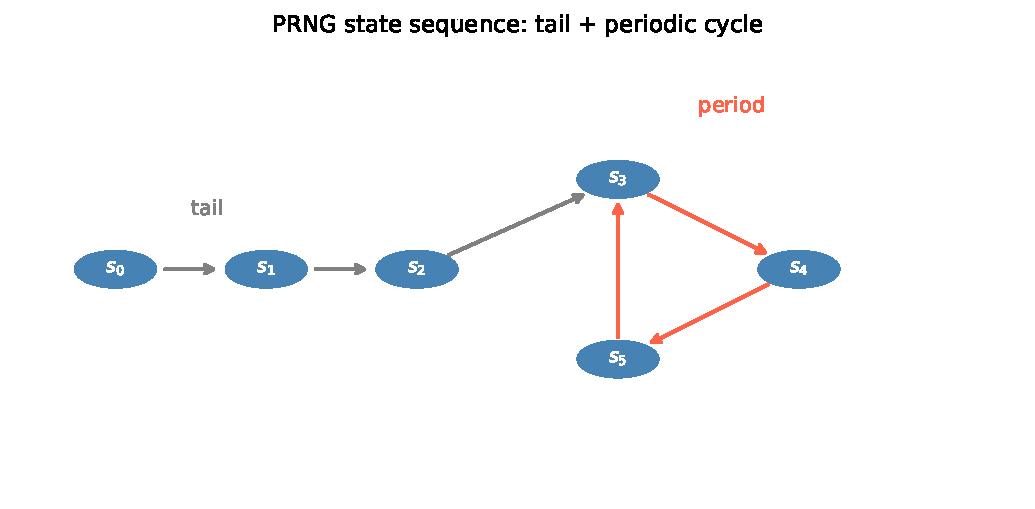
\includegraphics[width=0.55\textwidth]{prng_period}
\end{center}

The period cannot exceed $|S|$.

\end{frame}

%% ------------------------------------------------------------------
\begin{frame}[allowframebreaks]{2.1.1 Formal Definition: Random Numbers}

\textbf{Three types of random sequences used in Monte Carlo:}

\medskip
\begin{block}{Sequence of random numbers from $[0,1)$}
$U_1, U_2, \ldots$ where each $U_j \sim \mathcal{U}[0,1)$, i.e.,
\[
  \mathbb{P}(U_j \le t) = \begin{cases} 0 & t < 0,\\ t & 0 \le t < 1,\\ 1 & t \ge 1,\end{cases}
\]
\textbf{and} $U_1, U_2, \ldots$ are i.i.d.:
\[
  \mathbb{P}(U_1 \le t_1, \ldots, U_n \le t_n) = t_1 t_2 \cdots t_n, \quad 0\le t_i\le 1.
\]
\end{block}

\framebreak

\begin{block}{Sequence of random bits}
$B_1, B_2, \ldots$ where $B_j \in \{0,1\}$, i.i.d., with
\[
  \mathbb{P}(B_j = 0) = \mathbb{P}(B_j = 1) = \tfrac{1}{2}, \quad
  \mathbb{P}(B_1=b_1,\ldots,B_n=b_n) = \frac{1}{2^n}.
\]
\end{block}

\begin{block}{Sequence of random integers from $\bar{M}$}
$Y_1, Y_2, \ldots$ where $Y_j \in \{0,1,\ldots,M-1\} =: \bar{M}$, i.i.d.,
each uniformly distributed on $\bar{M}$.
\end{block}

\medskip
\textbf{Notation:} We write $U \sim \mathcal{U}(0,1)$, $B \sim \mathcal{U}(\{0,1\})$,
$Y \sim \mathcal{U}(\bar{M})$.

\medskip
PRNGs generate \emph{pseudorandom numbers}: deterministic sequences that
\emph{mimic} statistical properties of true random sequences.

\end{frame}

%% ==================================================================
\begin{frame}[allowframebreaks]{2.2 Random Permutations}

\textbf{Goal:} Generate a uniformly random permutation of $\{1,\ldots,n\}$,
i.e., each of the $n!$ arrangements has equal probability $1/n!$.

\medskip
\begin{block}{Algorithm 1: Fisher-Yates (Knuth Shuffle)}
\textbf{Input:} Integer $n$; pseudorandom numbers $\mathbf{u}=(u_1,\ldots,u_n)$,
$u_i\in[0,1)$\\
\textbf{Output:} A random permutation of $\{1,\ldots,n\}$
\begin{enumerate}
  \item Initialize: $S[i] = i$ for $i=1,\ldots,n$
  \item \textbf{for} $i = n$ downto $1$ \textbf{do}
  \item \quad $k = 1 + \lfloor i u_i \rfloor$ \hfill (pick random position in $\{1,\ldots,i\}$)
  \item \quad Swap$(S[k], S[i])$
  \item \textbf{end for}
  \item \textbf{return} $S$
\end{enumerate}
\end{block}

\begin{center}
  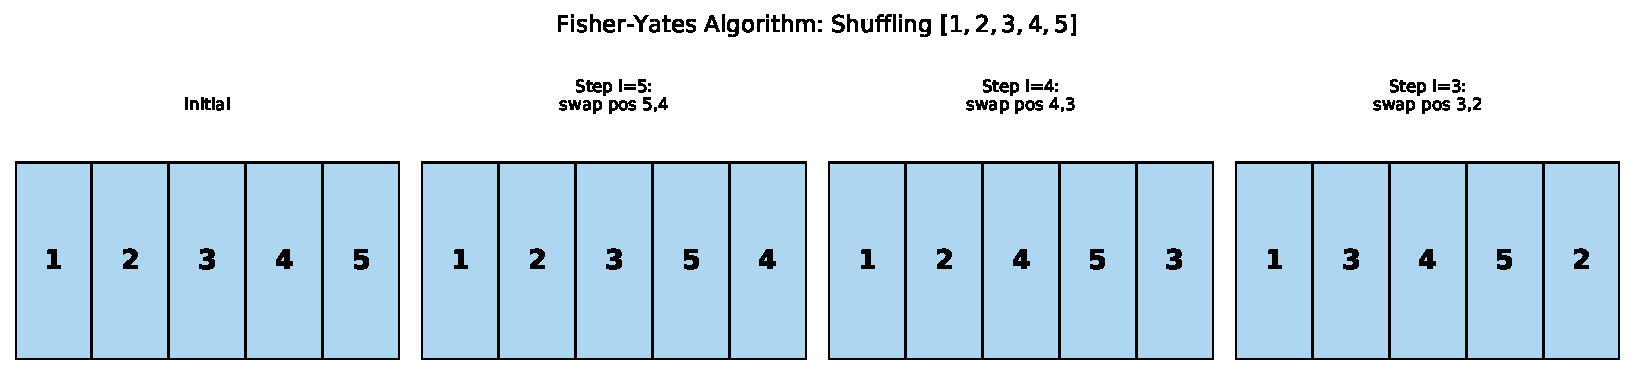
\includegraphics[width=0.80\textwidth]{fisher_yates}
\end{center}

\framebreak

\begin{block}{Algorithm 2: Perm-Sort}
An alternative: sort indices by $u_i$ values.
\begin{enumerate}
  \item $S[i] = i$ for $i=1,\ldots,n$
  \item Sort indices in $S$ such that $u_{S[1]} \le u_{S[2]} \le \cdots \le u_{S[n]}$
  \item \textbf{return} $S$
\end{enumerate}
\end{block}

Both algorithms produce a uniform random permutation, given a uniform input sequence.

\medskip
\textbf{Correctness of Fisher-Yates:} At step $i$, the element placed in position
$i$ is chosen uniformly from the remaining $i$ elements. This inductively yields a
uniform random permutation.

\end{frame}

%% ------------------------------------------------------------------
\begin{frame}[allowframebreaks]{2.2.2 Shuffling Cards}

\textbf{Physical analogy:} Shuffling a deck of 52 cards.
\begin{itemize}
  \item 52 cards $\Leftrightarrow$ $n = 52$
  \item Each arrangement has probability $1/52!$
  \item $52! \approx 8.07 \times 10^{67}$ possible orderings
\end{itemize}

\medskip
\textbf{Card Shuffling Schemes:}
\begin{itemize}
  \item \textbf{Top-To-Random:} Take the top card, insert it at a uniformly random position.
  \item \textbf{Riffle Shuffle:} Split deck into two roughly equal halves; interleave by
    dropping cards with probability proportional to pile size.
  \item \textbf{Time-Reversed Riffle Shuffle:} The reverse operation.
\end{itemize}

\framebreak

\textbf{How many shuffles to reach uniformity?}

After $k$ steps, the distribution of $X_k$ (the deck permutation) is compared to
the uniform distribution using the \emph{total variation distance}:
\[
  d_k = \frac{1}{2} \sum_{\sigma \in \mathcal{S}_n}
        \left|\mathbb{P}(X_k = \sigma) - \frac{1}{n!}\right|.
\]
As $k \to \infty$, $d_k \to 0$ (mixing property of Markov chains).

\medskip
\textbf{Key result (Bayer \& Diaconis):} For $n=52$ cards, approximately
\textbf{7 riffle shuffles} are needed before the deck is close to random.
Fewer shuffles leave detectable structure.

\end{frame}

%% ==================================================================
\begin{frame}[allowframebreaks]{2.3 Pseudorandom Number Generators in Python}

\textbf{Modern Python (NumPy):} The recommended approach uses \texttt{numpy.random}.

\medskip
\begin{block}{2.3.1 Python Generator Hierarchy}
\begin{itemize}
  \item \texttt{default\_rng(seed)} --- creates a Generator with PCG64 (default)
  \item \texttt{PCG64(seed)} --- Permuted Congruential Generator (64-bit)
  \item \texttt{MT19937(seed)} --- Mersenne Twister (legacy, period $2^{19937}-1$)
  \item \texttt{Philox}, \texttt{SFC64} --- alternative high-quality generators
\end{itemize}
\end{block}

\medskip
\textbf{PCG64 properties:}
\begin{itemize}
  \item Period: $2^{128}$ (essentially unlimited)
  \item Passes all standard statistical tests
  \item Multiple independent streams possible
  \item Recommended for Monte Carlo simulations
\end{itemize}

\framebreak

\textbf{MT19937 (Mersenne Twister):}
\begin{itemize}
  \item Period: $2^{19937} - 1$ (extremely long)
  \item State space: 624 32-bit integers
  \item Widely used historically (Python's \texttt{random} module, older NumPy)
  \item Fails some modern statistical tests
  \item Not suitable for cryptographic use
\end{itemize}

\medskip
\textbf{Getting random numbers from $\{0,\ldots,M-1\}$:}
Given $u_i \in [0,1)$, compute $y_i = \lfloor M u_i \rfloor$.

\end{frame}

%% ------------------------------------------------------------------
\begin{frame}[fragile]{2.3.1 Python Code: Using PRNGs}

\begin{lstlisting}[style=python]
import numpy as np

# Create a generator (PCG64 is the default)
rng = np.random.default_rng(seed=42)

# Generate n=10 uniform random numbers in [0, 1)
u = rng.random(10)
print("Uniform [0,1):", u)

# Generate integers in {0, 1, ..., 9}
y = rng.integers(0, 10, size=10)
print("Integers:", y)

# Fisher-Yates shuffle of [0,...,n-1]
n = 52
perm = rng.permutation(n)
print("Permutation:", perm[:10], "...")

# Explicitly use PCG64 or MT19937
from numpy.random import PCG64, MT19937, Generator
rng_pcg = Generator(PCG64(seed=0))
rng_mt  = Generator(MT19937(seed=0))

# Compare outputs
print("PCG64:", rng_pcg.random(5))
print("MT19937:", rng_mt.random(5))
\end{lstlisting}

\end{frame}

%% ------------------------------------------------------------------
\begin{frame}[allowframebreaks]{2.3.2 Cryptographic PRNGs: RC4}

\textbf{Cryptographic PRNGs} must satisfy:
\begin{itemize}
  \item All standard statistical tests (like non-cryptographic PRNGs)
  \item \textbf{In addition:} computationally infeasible to predict future/past
    outputs given partial observations
\end{itemize}

\medskip
\textbf{Definition:} A PRNG is \emph{cryptographically secure} (CSPRNG) if no
polynomial-time algorithm can distinguish its output from a truly random sequence
with non-negligible advantage.

\medskip
\textbf{RC4 (Rivest Cipher 4):}
\begin{itemize}
  \item Stream cipher designed in 1987 by Ron Rivest (RSA Security)
  \item Based on a \emph{key-scheduling algorithm} (KSA) and a
    \emph{pseudo-random generation algorithm} (PRGA)
  \item Was widely used in TLS/SSL, WEP, PDF encryption
  \item Now considered \emph{insecure} --- deprecated in TLS 1.3
\end{itemize}

\framebreak

\begin{block}{RC4: Key-Scheduling Algorithm (KSA)}
\textbf{Input:} $n$, key $K[0],\ldots,K[L-1]$\\
\textbf{Output:} Permutation $S[0],\ldots,S[n-1]$
\begin{enumerate}
  \item Initialize: $S[i] = i$ for $i=0,\ldots,n-1$
  \item $j := 0$
  \item \textbf{for} $i=0$ to $n-1$ \textbf{do:}
  \quad $j = (j + S[i] + K[i \bmod L]) \bmod n$;
  \quad Swap$(S[i], S[j])$
\end{enumerate}
\end{block}

\begin{block}{RC4: Pseudo-Random Generation Algorithm (PRGA)}
\textbf{Input:} $S[0],\ldots,S[n-1]$ (from KSA)\\
\textbf{Output:} Bytes $x_1, x_2, \ldots$
\begin{itemize}
  \item $i := 0$, $j := 0$
  \item \textbf{while} generating output \textbf{do:}
    $i = (i+1) \bmod n$;
    $j = (j + S[i]) \bmod n$;
    Swap$(S[i], S[j])$;
    $x_r = S[(S[i]+S[j]) \bmod n]$
\end{itemize}
\end{block}

\framebreak

\begin{center}
  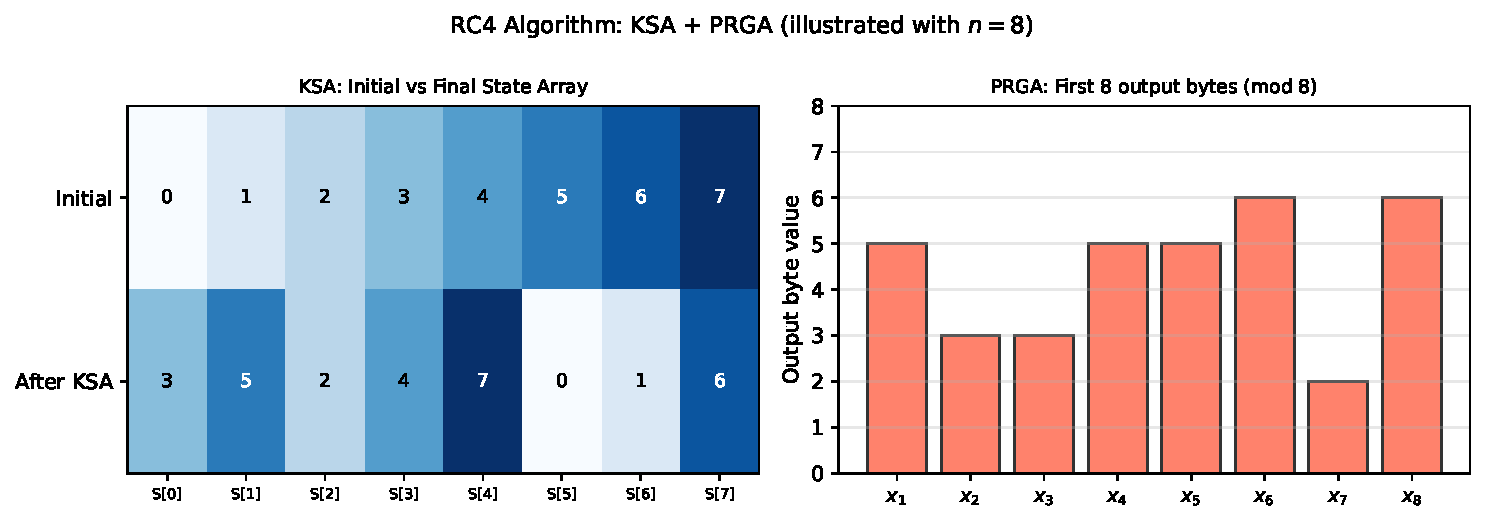
\includegraphics[width=0.70\textwidth]{rc4_schematic}
\end{center}

\textbf{Security note:} RC4 has known biases in the first few bytes of output
and statistical weaknesses discovered by Fluhrer, Mantin, and Shamir (2001).
The IETF deprecated it in RFC 7465.

\end{frame}

%% ------------------------------------------------------------------
\begin{frame}[fragile]{2.3.2 Python Code: RC4 Implementation}

\begin{lstlisting}[style=python]
def rc4_ksa(n, key):
    """Key-Scheduling Algorithm."""
    S = list(range(n))
    j = 0
    L = len(key)
    for i in range(n):
        j = (j + S[i] + key[i % L]) % n
        S[i], S[j] = S[j], S[i]
    return S

def rc4_prga(S, num_bytes):
    """Pseudo-Random Generation Algorithm."""
    n = len(S); i = j = 0; output = []
    while len(output) < num_bytes:
        i = (i + 1) % n
        j = (j + S[i]) % n
        S[i], S[j] = S[j], S[i]
        t = (S[i] + S[j]) % n
        output.append(S[t])
    return output

# Example: 256-element state, key = [3, 1, 4, 1, 5]
key = [3, 1, 4, 1, 5]
S = rc4_ksa(256, key)
stream = rc4_prga(S, 20)
print("RC4 keystream:", stream)
\end{lstlisting}

\end{frame}

%% ==================================================================
\begin{frame}[allowframebreaks]{2.4 Simple Generators: Historical Perspective}

\textbf{Overview:} Before modern PRNGs, several simple generators were widely used.
They are primarily of \emph{historical and educational} value:
\begin{itemize}
  \item Easy to implement and analyze mathematically
  \item Typically 32-bit with limited period
  \item Poor statistical quality by modern standards
  \item Vulnerable to predictability attacks
\end{itemize}

\medskip
Understanding them builds intuition for PRNG design challenges.

\end{frame}

%% ------------------------------------------------------------------
\begin{frame}[allowframebreaks]{2.4.1 Linear Congruential Generators (LCG)}

\begin{block}{Linear Congruential Recurrence}
\[
  x_{n+1} = (a x_n + c) \bmod M \tag{2.4.1}
\]
Parameters:
\begin{itemize}
  \item $M > 0$: \textbf{modulus}
  \item $0 \le a < M$: \textbf{multiplier}
  \item $0 \le c < M$: \textbf{increment}
  \item $0 \le x_0 < M$: \textbf{seed}
\end{itemize}
Output: $u_n = x_n / M \in [0,1)$
\end{block}

\medskip
The period cannot exceed $M$. Good choice of parameters gives period exactly $M$.

\framebreak

\begin{block}{Theorem 2.4.1 (Full Period Conditions)}
Let $b = a - 1$. The sequence $(x_n)$ has period $M$ if and only if:
\begin{itemize}
  \item $c$ is coprime with $M$,
  \item $b$ is a multiple of $p$ for every prime $p$ dividing $M$,
  \item If $4$ divides $M$, then $a \equiv 1 \pmod{4}$.
\end{itemize}
\end{block}

\medskip
\textbf{Historical examples:}

\begin{description}
  \item[Example 2.4.2] $M = 2^{31}-1 = 2147483647$, $a = 7^5 = 16807$, $c = 0$.\\
    Period $= M - 1$ (prime modulus). Also: $M = 2^{31}-1$, $a = 40014$.
  \item[Example 2.4.3 (Resing)] $(a,c,M) = (1,5,13)$, $x_0 = 1$:\\
    Sequence: $1, 6, 11, 3, 8, 0, 5, 10, 2, 7, 12, 4, 9, 1, \ldots$, period 13.
  \item[Example 2.4.3] $(a,c,M) = (2,5,13)$, $x_0 = 1$:\\
    Sequence: $1, 7, 6, 4, 0, 5, 2, 9, \ldots$, period 12.
    If $x_0 = 8$: constant sequence (period 1).
\end{description}

\framebreak

\begin{center}
  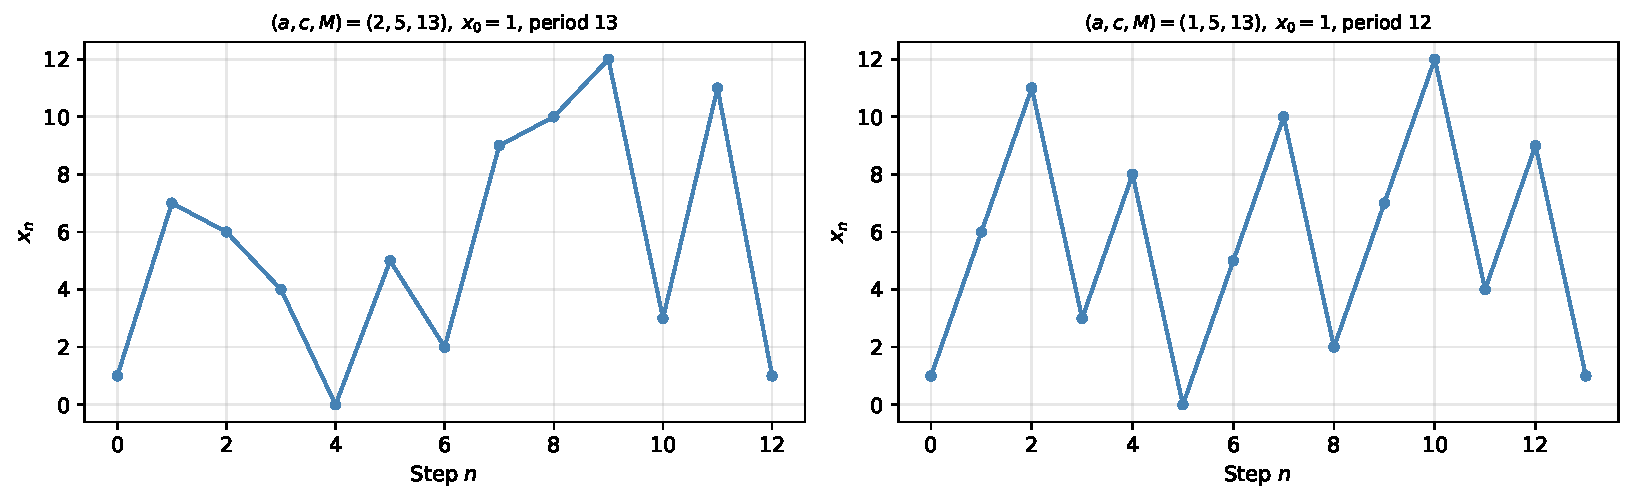
\includegraphics[width=0.85\textwidth]{lcg_sequences}
\end{center}

\begin{center}
  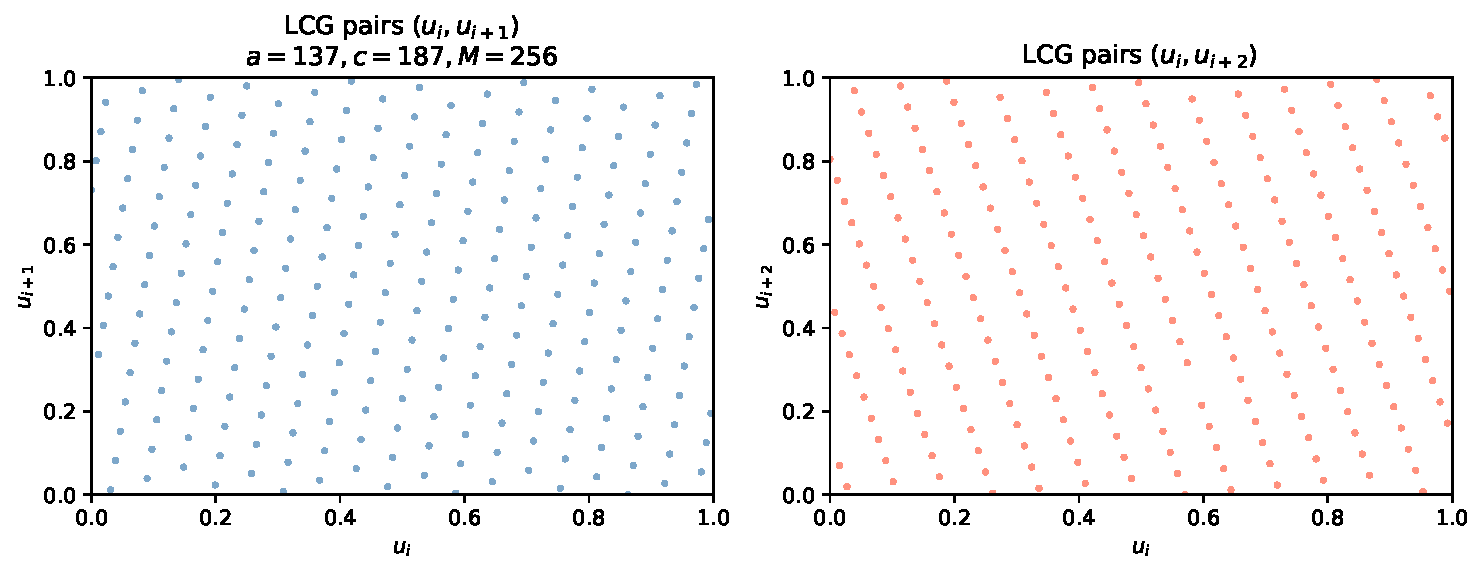
\includegraphics[width=0.85\textwidth]{lcg_pairs}
\end{center}

Note the \emph{lattice structure} in pairs $(u_i, u_{i+1})$ ---
a known weakness of LCGs.

\framebreak

\textbf{Commercial LCG parameters:}

\medskip
\begin{tabular}{lll}
  \toprule
  System & Recurrence & Output \\
  \midrule
  \textbf{Java} & $x_{i+1} = (25214903917\,x_i + 11) \bmod 2^{48}$ & $u_i = (2^{27}\lfloor x_{2i}/2^{22}\rfloor + \lfloor x_{2i+1}/2^{21}\rfloor)/2^{53}$ \\
  \textbf{Visual Basic} & $x_i = (1140671485\,x_{i-1} + 12820163)\bmod 2^{24}$ & $u_i = x_i/2^{24}$ \\
  \textbf{Excel} & $u_i = (0.9821\,u_{i-1} + 0.211327)\bmod 1$ & --- \\
  \textbf{rand48} (UNIX) & Same as Java for $x_i$ & $u_i = x_i/2^{48}$ \\
  \bottomrule
\end{tabular}

\medskip
These fail modern statistical tests and should \emph{not} be used for serious simulations.

\framebreak

\textbf{Generalized Linear Congruential Generator:}
\[
  x_n = (a_1 x_{n-1} + a_2 x_{n-2} + \cdots + a_k x_{n-k} + c) \bmod M.
\]
Achieves period up to $M^k$ with appropriate coefficients.

\medskip
\textbf{Quadratic Congruential Generator I (QCG I):}
\[
  x_{i+1} = x_i^2 \bmod M,
\]
where $M$ is a 512-bit prime.

\medskip
\textbf{Quadratic Congruential Generator II (QCG II):}
\[
  x_{i+1} = 2x_i^2 + 3x_i + 1 \bmod 2^{512}.
\]

\textbf{Cubic Congruential Generator (CCG):}
\[
  x_{i+1} = 2x_i^3 \bmod 2^{512}.
\]

\textbf{Fibonacci Generator:}
\[
  x_n = x_{n-1} + x_{n-2} \bmod M \quad (n \ge 2).
\]

\textbf{Lagged Fibonacci (Knuth):}
\[
  x_n = x_{n-k} + x_{n-l} \bmod M, \quad n \ge \max(k,l),
\]
with $k=100$, $l=37$, $M=2^{30}$ (Knuth's recommended parameters).

\end{frame}

%% ------------------------------------------------------------------
\begin{frame}[fragile]{2.4.1 Python Code: LCG Implementation}

\begin{lstlisting}[style=python]
import numpy as np
import matplotlib.pyplot as plt

def lcg(a, c, M, x0, n):
    """Linear Congruential Generator."""
    x = x0
    seq = []
    for _ in range(n):
        x = (a * x + c) % M
        seq.append(x / M)
    return seq

# Example 2.4.3: (a,c,M) = (2,5,13), x0 = 1, period = 12
u1 = lcg(a=2, c=5, M=13, x0=1, n=14)
print("LCG (2,5,13), x0=1:", [round(x,3) for x in u1])

# Compare with PCG64
rng = np.random.default_rng(seed=0)
u_pcg = rng.random(14)
print("PCG64:", [round(x,3) for x in u_pcg])

# Plot pairs to see lattice structure
u = lcg(a=137, c=187, M=256, x0=1, n=256)
plt.figure(figsize=(5,4))
plt.scatter(u[:-1], u[1:], s=4, alpha=0.7)
plt.title('LCG pairs: lattice structure visible')
plt.xlabel(r'$u_i$'); plt.ylabel(r'$u_{i+1}$')
plt.tight_layout(); plt.savefig('lcg_scatter.pdf')
\end{lstlisting}

\end{frame}

%% ------------------------------------------------------------------
\begin{frame}[allowframebreaks]{2.4.1 L'Ecuyer Mixed Generator}

\textbf{Idea:} Combine two LCGs to get much longer period and better quality.

\begin{block}{L'Ecuyer Mixed Generator}
\begin{enumerate}
  \item $x_n = (A_1 x_{n-2} - A_2 x_{n-3}) \bmod M_1$
  \item $y_n = (B_1 y_{n-1} - B_2 y_{n-3}) \bmod M_2$
  \item $z_n = (x_n - y_n) \bmod M_1$
  \item $u_n = z_n/(M_1+1)$ if $z_n > 0$; otherwise $u_n = M_1/(M_1+1)$
\end{enumerate}
Parameters: $M_1 = 4294967087$, $M_2 = 4294944443$,\\
$A_1 = 1403580$, $A_2 = 810728$, $B_1 = 527612$, $B_2 = 1370589$.
\end{block}

Period $\approx 2^{191}$, passing many statistical tests. This was state-of-the-art
before PCG64/MT19937.

\end{frame}

%% ------------------------------------------------------------------
\begin{frame}[allowframebreaks]{2.4.2 Bit Generators}

Sequences of $\{0,1\}$-valued pseudorandom numbers are \textbf{pseudorandom bits}.

\medskip
\textbf{Register operations:}
\begin{itemize}
  \item \textbf{XOR} ($\oplus$): $p \oplus q = 1$ iff an odd number of inputs is 1.
    \[
      \mathbf{p} \oplus \mathbf{q} = (p_1 \oplus q_1, \ldots, p_n \oplus q_n).
    \]
  \item \textbf{Bit shifts}: $\ll$ (left shift), $\gg$ (right shift). For example,
    $x = y \ll 2$ shifts $y$ left by 2 positions (fills with zeros).
\end{itemize}

\medskip
\textbf{XOR truth table:}
\begin{center}
\begin{tabular}{cc|c}
$p$ & $q$ & $p \oplus q$ \\
\hline
0 & 0 & 0 \\
0 & 1 & 1 \\
1 & 0 & 1 \\
1 & 1 & 0 \\
\end{tabular}
\end{center}

\framebreak

\begin{block}{XORG: Exclusive OR Generator}
\[
  x_i = x_{i-1} \oplus x_{i-127}, \quad i \ge 128,
\]
initialized with a 127-bit seed. Simple and fast.
\end{block}

\begin{block}{LFSR: Linear Feedback Shift Register}
\[
  x_i = (a_1 x_{i-1} \oplus a_2 x_{i-2} \oplus \cdots \oplus a_k x_{i-k}),
\]
where $a_j \in \{0,1\}$ are \textbf{feedback taps}. With appropriate taps,
achieves maximum period $2^k - 1$.
\end{block}

\begin{center}
  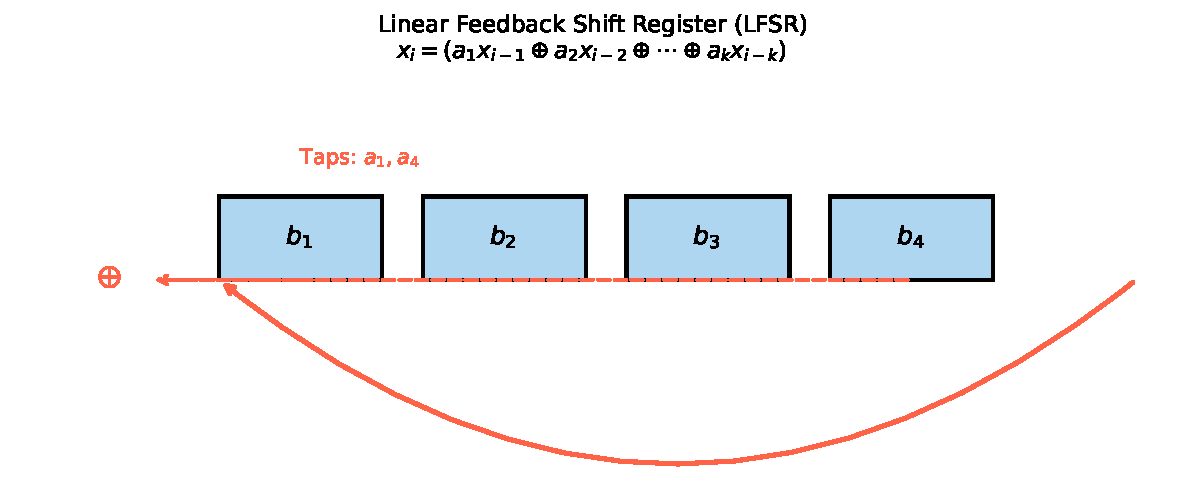
\includegraphics[width=0.65\textwidth]{lfsr_schematic}
\end{center}

\framebreak

\begin{block}{Blum-Blum-Shub (BBS) Generator}
\[
  x_{i+1} = x_i^2 \bmod M, \quad M = pq \text{ (product of two large primes)}.
\]
Output: the least significant bit of $x_i$.\\
\emph{Cryptographically secure} under the quadratic residuosity assumption,
but slow for Monte Carlo use.
\end{block}

\begin{block}{Shift-XOR (SXR) Generator}
\begin{enumerate}
  \item Seed $x_0 \in \{0,1,\ldots,2^n-1\}$ ($n=32$ or $n=64$)
  \item $x_{i+1} = (x_i \oplus (x_i \ll a)) \oplus (x_i \gg b)$
  \item Output $x_{i+1}$
\end{enumerate}
For $n=32$: $a=13$, $b=17$ gives a simple efficient generator.\\
Example: $x_0 = \texttt{0xABCDE123}$:
\[
  x_1 = (x_0 \oplus (x_0 \ll 13)) \oplus (x_0 \gg 17), \quad \ldots
\]
\end{block}

Properties: (i) simple bitwise implementation; (ii) short period; (iii) good
randomness for simple uses but fails advanced tests.

\end{frame}

%% ==================================================================
\begin{frame}[allowframebreaks]{2.5 Testing Good Properties of PRNGs}

\textbf{Two types of tests:}
\begin{enumerate}
  \item \textbf{Theoretical tests}: examine internal generator structure (e.g.,
    lattice tests, spectral tests). Detect structural weaknesses without running the generator.
  \item \textbf{Statistical tests}: treat the PRNG as a black box; run it and apply
    hypothesis tests to the output.
\end{enumerate}

\medskip
\textbf{Test batteries:}
\begin{itemize}
  \item \textbf{Diehard} tests (Marsaglia): 18 tests; widely used historically
  \item \textbf{TestU01} (L'Ecuyer \& Simard): comprehensive suite; small/medium/big crush
  \item \textbf{NIST SP 800-22} (National Institute of Standards and Technology):
    15 tests for cryptographic applications
  \item \textbf{Uniformity}, \textbf{Scalability}, \textbf{Consistency}:
    basic requirements for any good PRNG
\end{itemize}

\medskip
\textbf{Motivating experiment:} Generate 256 pairs $(x_i, x_{i+1})$ for the LCG
$x_j = (137 x_{j-1} + 187) \bmod 256$. Plot the pairs and triples. The lattice
structure is immediately visible (see LCG pairs figure above).

\end{frame}

%% ------------------------------------------------------------------
\begin{frame}[allowframebreaks]{2.5.1 Preliminary Remarks}

\textbf{Notation:}
\begin{itemize}
  \item $U \sim \mathcal{U}(0,1)$: uniform on $[0,1)$
  \item $B \sim \mathcal{U}(\{0,1\})$: uniform random bit
  \item $Y \sim \mathcal{U}(\bar{M})$: uniform on $\{0,\ldots,M-1\}$
\end{itemize}

\medskip
\begin{block}{Converting Between Formats (2.5.1)}
\textbf{From $[0,1)$ to $\bar{M}$:}
\[
  y_i = \lfloor M u_i \rfloor.
\]
\textbf{From $\bar{M}$ to $[0,1)$:}
\[
  u_i = y_i / M.
\]
\textbf{From $[0,1)$ to bits (careful method):}
First convert $u_i \to y_i \in \bar{M}$ (with $M = 2^k$), then use binary expansion of $y_i$.
\end{block}

\medskip
\textbf{Warning:} The naive conversion $b_i = \mathbb{1}[u_i \ge 0.5]$ discards
all but the most significant bit, and can be exploited to cheat tests.

\framebreak

\begin{block}{Grouping into Multidimensional Vectors (2.5.1.2)}
Given $n = mr$ numbers $u_1,\ldots,u_n$, group into $r$ vectors of length $m$:
\[
  \mathbf{u}_1 = (u_1,\ldots,u_m), \quad
  \mathbf{u}_2 = (u_{m+1},\ldots,u_{2m}), \quad
  \ldots, \quad
  \mathbf{u}_r = (u_{(r-1)m+1},\ldots,u_{rm}).
\]
Each $\mathbf{u}_i \in [0,1)^m$. Similarly for integer sequences: $\mathbf{y}_i \in \bar{M}^m$.
\end{block}

\medskip
\begin{block}{The p-value concept (2.5.1.3)}
\[
  p = \mathbb{P}(T \ge T(\text{obs})) = 1 - F(T(\text{obs})),
\]
where $T$ is the test statistic and $F$ is its c.d.f. under $\mathcal{H}_0$.
\begin{itemize}
  \item Under $\mathcal{H}_0$: $p \sim \mathcal{U}(0,1)$
  \item Small $p$ (e.g., $< 0.01$): evidence \emph{against} randomness
  \item Large $p$ (e.g., $> 0.99$): suspiciously ``too perfect'' (quasi-random)
\end{itemize}
\end{block}

\begin{center}
  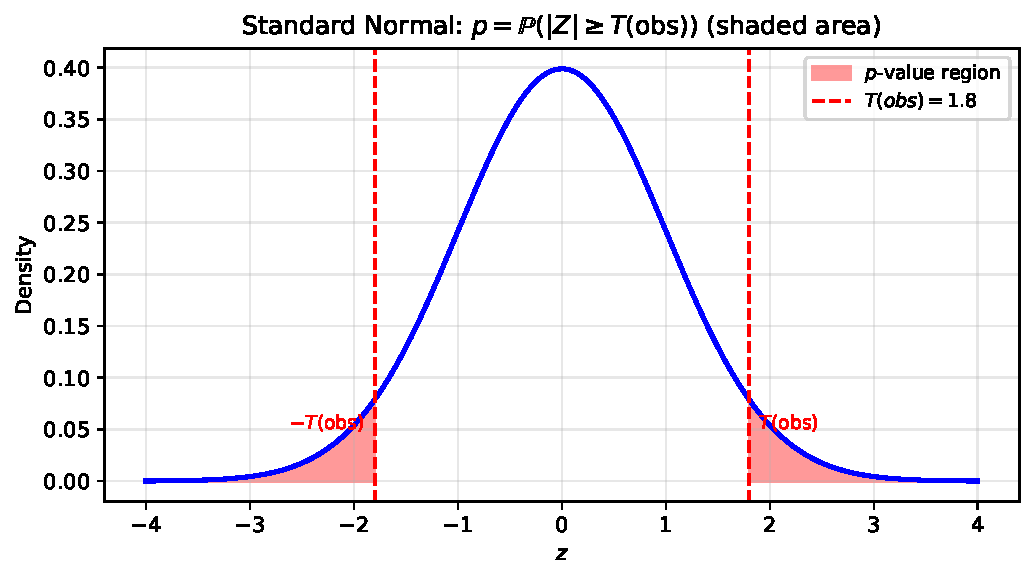
\includegraphics[width=0.55\textwidth]{normal_pvalue}
\end{center}

\end{frame}

%% ------------------------------------------------------------------
\begin{frame}[allowframebreaks]{2.5.2 Kolmogorov-Smirnov and Chi-Square Tests}

\textbf{Running example:} Three sets of $n=50$ points from $[0,1)$:
\begin{itemize}
  \item \textbf{Set A}: PCG64 (truly pseudorandom)
  \item \textbf{Set B}: Nonlinear transform of A (not uniform)
  \item \textbf{Set C}: Quasi-random (van der Corput / Halton sequence)
\end{itemize}

\begin{center}
  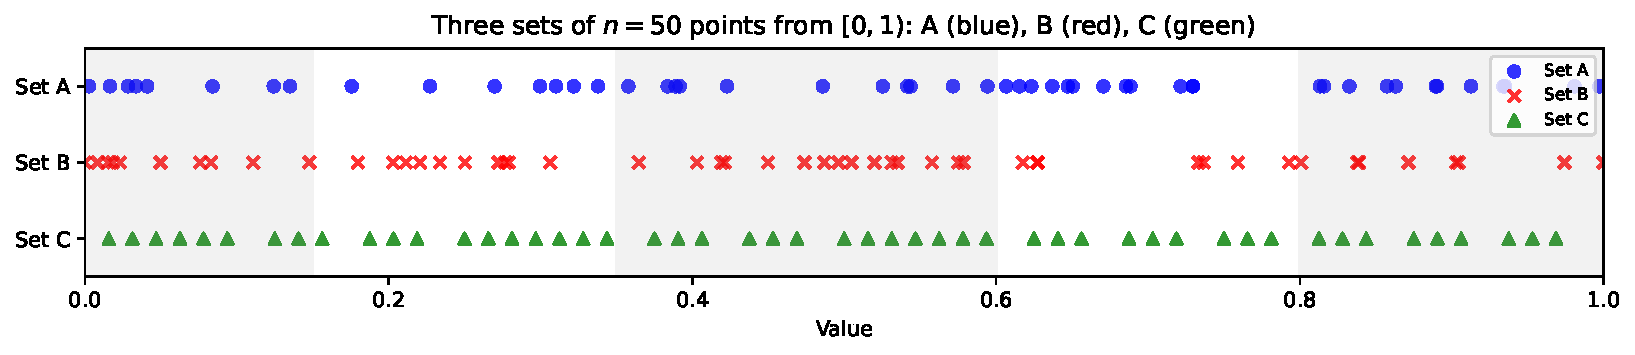
\includegraphics[width=0.85\textwidth]{sets_abc}
\end{center}

\framebreak

\begin{block}{Kolmogorov-Smirnov (KS) Test}
\textbf{Empirical CDF:}
\[
  \hat{F}_n(t) = \frac{1}{n}\sum_{i=1}^n \mathbb{1}(U_i \le t).
\]
\textbf{KS statistic:}
\[
  D_n = \sup_{0 \le t \le 1} |\hat{F}_n(t) - t|.
\]
Under $\mathcal{H}_0$ ($U_i \sim \mathcal{U}(0,1)$, i.i.d.): $D_n \to 0$ a.s. (Glivenko-Cantelli).\\
Moreover, $\sqrt{n} D_n$ converges to the \textbf{Kolmogorov distribution}:
\[
  K(t) = \lim_{n\to\infty} \mathbb{P}(\sqrt{n}D_n \le t)
       = 1 - 2J(\exp(-2t^2)), \quad t > 0,
\]
where $J(t) = \sum_{j=1}^\infty (-1)^{j-1}\exp(-2j^2 t^2)$.
\end{block}

\textbf{Critical values:}
$\lambda_{0.1} = 1.224$, $\lambda_{0.05} = 1.358$, $\lambda_{0.01} = 1.628$.

\framebreak

\textbf{Computing $D_n$ from order statistics:}
Let $U_{(1)} \le \cdots \le U_{(n)}$ be the sorted sample. Then:
\[
  D_n^+ = \max_{1\le i\le n}\left(\frac{i}{n} - U_{(i)}\right), \quad
  D_n^- = \max_{1\le i\le n}\left(U_{(i)} - \frac{i-1}{n}\right), \quad
  D_n = \max(D_n^+, D_n^-).
\]

\textbf{p-value formula} (with correction for finite $n$):
\[
  p = 1 - K\!\left(\sqrt{n}\,D_n(\text{obs}) + \frac{1}{6\sqrt{n}} + \frac{\sqrt{n}D_n(\text{obs})-1}{4n}\right).
\]

\begin{center}
  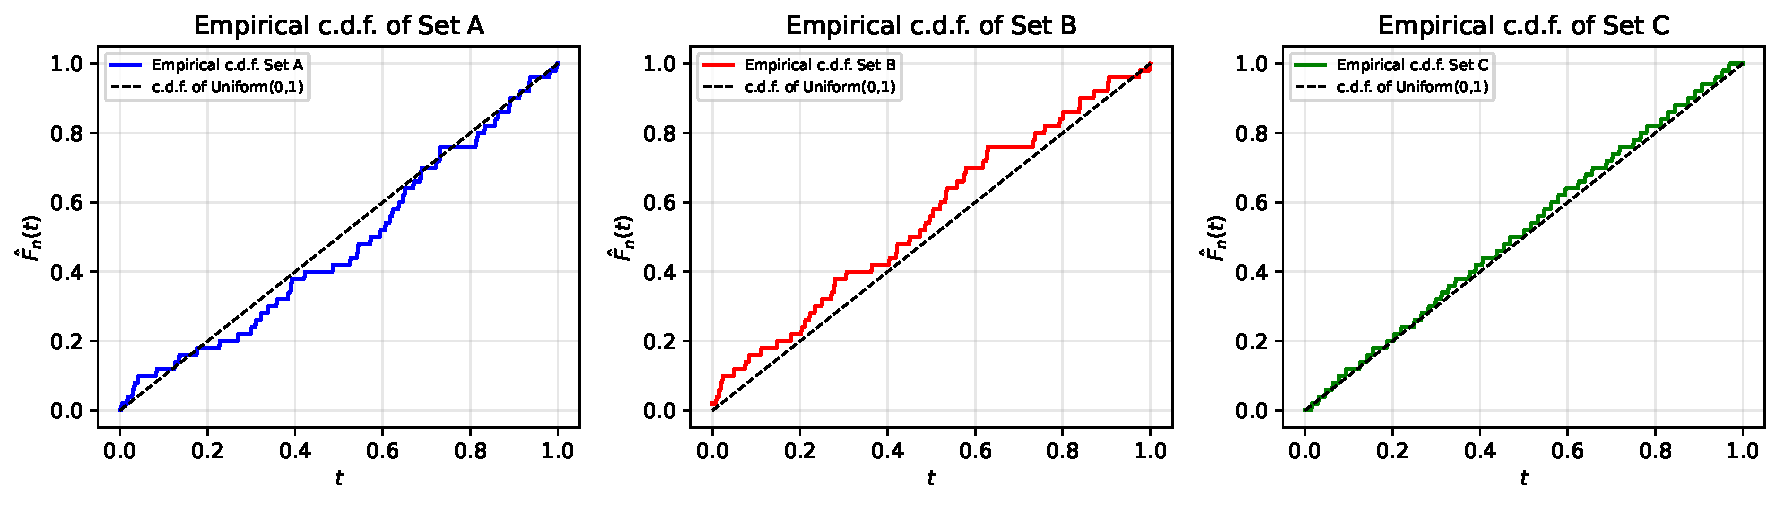
\includegraphics[width=0.90\textwidth]{ecdf_abc}
\end{center}

\framebreak

\begin{center}
  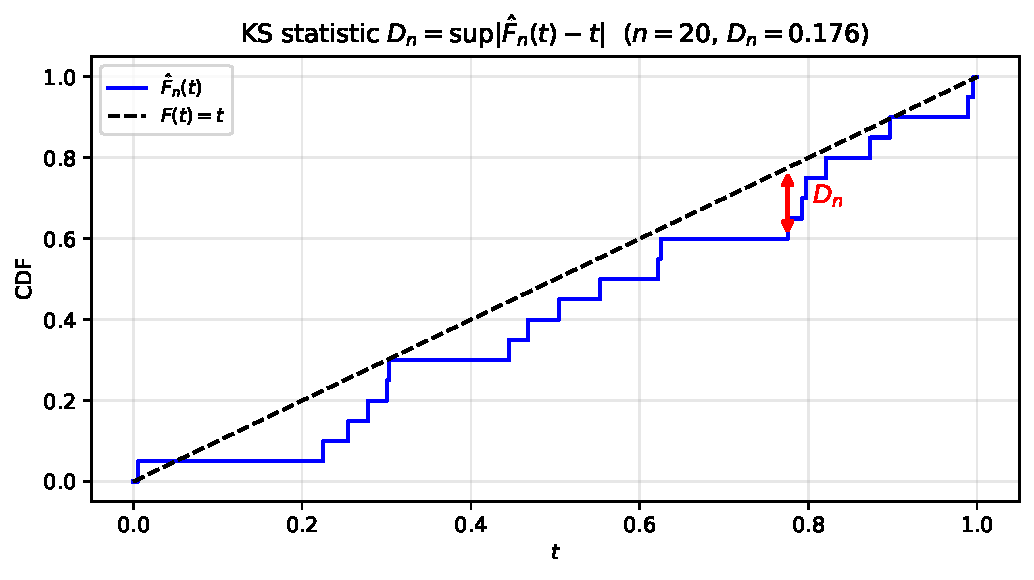
\includegraphics[width=0.60\textwidth]{ks_illustration}
\end{center}

\textbf{KS test results for Sets A, B, C} (Example 2.5.1, $n=50$):
\begin{center}
\begin{tabular}{lccc}
  \toprule
  & Set A & Set B & Set C \\
  \midrule
  $D_n(\text{obs})$ & 0.1192 & 0.2266 & 0.0462 \\
  $p$-value & 44.17\% & 0.99\% & 99.97\% \\
  Conclusion & Not rejected & \textbf{Rejected} & Not rejected\\
  \bottomrule
\end{tabular}
\end{center}

Set C (quasi-random) has suspiciously \emph{large} $p$-value: ``too uniform.''
Second-level testing detects this (see Sect.~2.5.6).

\framebreak

\begin{block}{Chi-Square Goodness-of-Fit Test}
Given $k$ classes with probabilities $p_1,\ldots,p_k$ and $r$ trials,
let $O_i$ = observed count in class $i$, $E_i = r p_i$ = expected count.
\[
  X_k^2 = \sum_{i=1}^k \frac{(O_i - r p_i)^2}{r p_i} = \sum_{i=1}^k \frac{O_i^2}{r p_i} - r.
\]
As $r \to \infty$: $X_k^2 \xrightarrow{\mathcal{D}} \chi^2_{k-1}$.\\
\textbf{Rule of thumb:} Each class needs at least 5 expected observations:
$r \ge \lceil 5 / \min_i p_i \rceil$.
\end{block}

\medskip
\textbf{Chi-square results for Sets A, B, C} (partition $\mathcal{P}$ into 5 bins, $r=50$):

\begin{center}
\begin{tabular}{lccc}
\toprule
& Set A & Set B & Set C \\
\midrule
$X^2(\text{obs})$ & 7.32 & 16.25 & 0.24 \\
$p$-value ($\chi^2_4$) & 11.99\% & 0.27\% & 99.35\% \\
\bottomrule
\end{tabular}
\end{center}

\begin{center}
  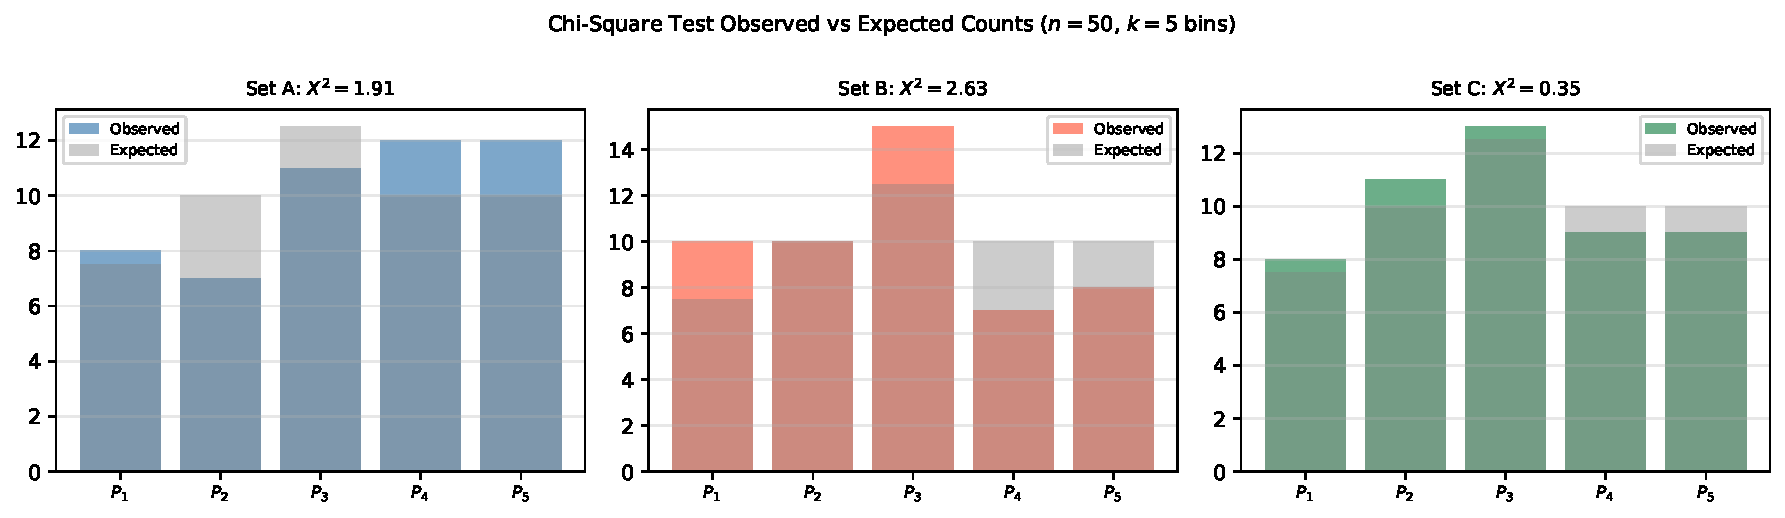
\includegraphics[width=0.85\textwidth]{chisq_hist}
\end{center}

\end{frame}

%% ------------------------------------------------------------------
\begin{frame}[fragile]{2.5.2 Python Code: KS and Chi-Square Tests}

\begin{lstlisting}[style=python]
import numpy as np
from scipy import stats

rng = np.random.default_rng(0)
n = 50
A = rng.random(n)

# Set B: exponential transform (non-uniform)
eps = 1e-7
B_raw = np.exp(A - 1) - 1 - eps
B = (B_raw - B_raw.min()) / (B_raw.max() - B_raw.min())

# Kolmogorov-Smirnov test
ks_stat_A, p_A = stats.kstest(A, 'uniform')
ks_stat_B, p_B = stats.kstest(B, 'uniform')
print(f"Set A: D={ks_stat_A:.4f}, p={p_A:.4f}")
print(f"Set B: D={ks_stat_B:.4f}, p={p_B:.4f}")

# Chi-square test with 5 equal bins
bins = [0, 0.2, 0.4, 0.6, 0.8, 1.0]
obs_A, _ = np.histogram(A, bins=bins)
exp    = [n/5] * 5
chi2_A, p_chi2_A = stats.chisquare(obs_A, exp)
obs_B, _ = np.histogram(B, bins=bins)
chi2_B, p_chi2_B = stats.chisquare(obs_B, exp)
print(f"Set A chi2: X2={chi2_A:.3f}, p={p_chi2_A:.4f}")
print(f"Set B chi2: X2={chi2_B:.3f}, p={p_chi2_B:.4f}")
\end{lstlisting}

\end{frame}

%% ------------------------------------------------------------------
\begin{frame}[allowframebreaks]{2.5.3 Tests Based on Balls-and-Boxes Schemes}

\textbf{General framework:} Place $r$ balls into $k$ boxes uniformly at random.
Under $\mathcal{H}_0$: each ball independently goes to box $i$ with probability $p_i = 1/k$.

\begin{center}
  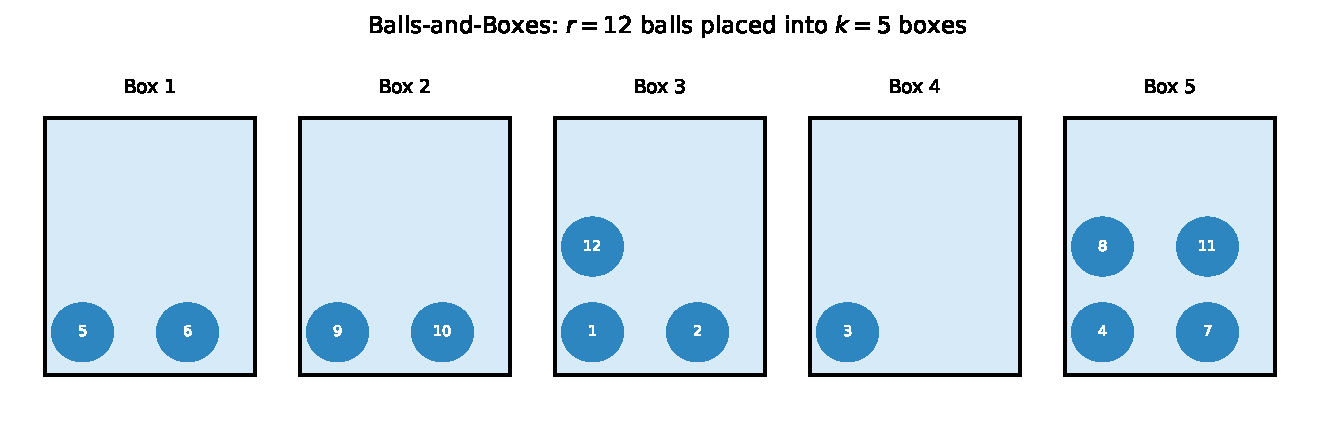
\includegraphics[width=0.70\textwidth]{balls_boxes}
\end{center}

\textbf{Birthday problem:} $r$ people, $k=365$ boxes (days).
\[
  p = 1 - \frac{(365)_r}{365^r} = 1 - \prod_{j=1}^{r-1}\left(1 - \frac{j}{365}\right).
\]
With $r=23$ people: $p \approx 0.507$. General approximation:
\[
  p_{k,r} \approx 1 - \exp\!\left(-\frac{r^2}{2k}\right). \tag{2.5.12}
\]

\begin{center}
  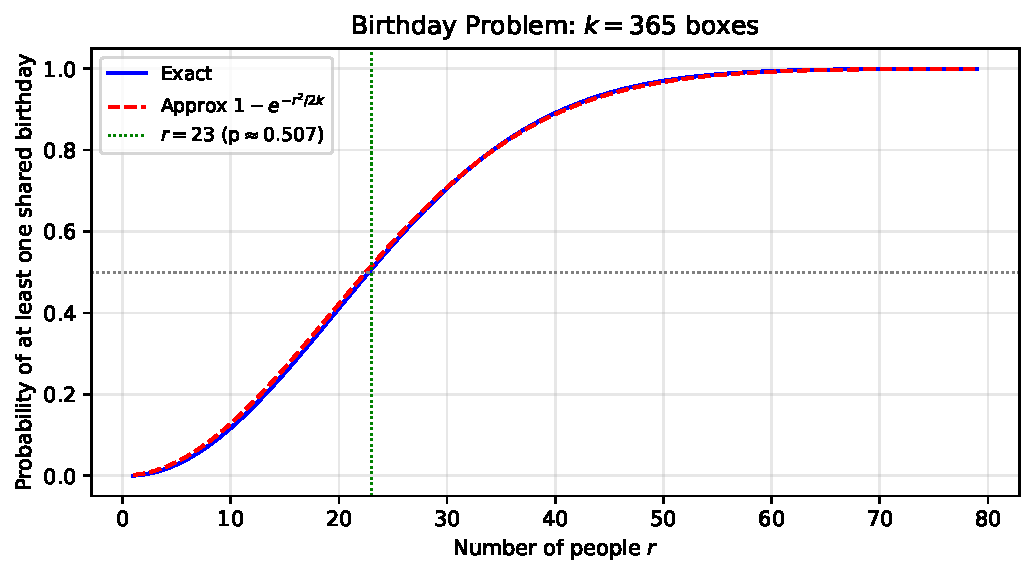
\includegraphics[width=0.60\textwidth]{birthday_problem}
\end{center}

\framebreak

\textbf{Converting a sequence to balls-and-boxes:}

Given $u_1,\ldots,u_n$ from $[0,1)$, group into $r$ vectors of length $m$:
\[
  \mathbf{u}_i = (u_{(i-1)m+1},\ldots,u_{im}), \quad i=1,\ldots,r.
\]
Divide $[0,1)^m$ into $k = L^m$ sub-hypercubes:
\[
  A_{q_1,\ldots,q_m} = \left\{(v_1,\ldots,v_m): v_i \in \left[\frac{q_i}{L}, \frac{q_i+1}{L}\right)\right\},
  \quad q_i \in \{0,\ldots,L-1\}.
\]
$\mathbf{u}_i$ falls into box $(q_1,\ldots,q_m)$: $y_j = \lfloor L u_j \rfloor$.

\medskip
\begin{block}{Collision Test}
Count $C_{k,r}$ = number of collisions (balls landing in occupied boxes).
\[
  \mathbb{P}(C_{k,r} = c) = \frac{k(k-1)\cdots(k-r+c+1)\,S_2(r, r-c)}{k^r}, \tag{2.5.13}
\]
where $S_2(r,s)$ = Stirling number of the second kind.\\
\textbf{Poisson approximation:} As $r, k \to \infty$ with $r^2/(2k) \to \lambda$:
\[
  \mathbb{P}(C_{k,r} = c) \to \frac{\lambda^c}{c!} e^{-\lambda}. \tag{2.5.14}
\]
\end{block}

\framebreak

\begin{block}{Expected Number of Collisions}
\[
  \mathbb{E} C_{k,r} = r - k\left(1 - \left(1-\frac{1}{k}\right)^r\right) \approx \frac{r^2}{2k}.
  \tag{2.5.17}
\]
For $r=2^{14}$ and $k=2^{20}$: $\mathbb{E} C_{k,r} \approx 128$.
\end{block}

\begin{center}
  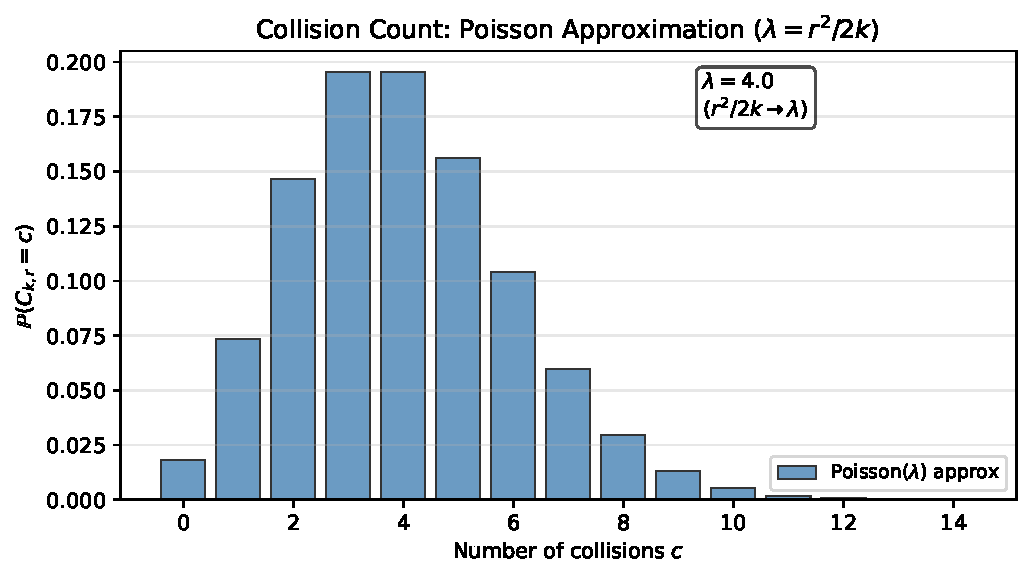
\includegraphics[width=0.60\textwidth]{collision_distribution}
\end{center}

\framebreak

\textbf{Spacing Test:} Consider spacings between occurrences of $U_j \in (\alpha, \beta]$.
\begin{itemize}
  \item $\delta = \beta - \alpha$; consecutive spacings $C_1, C_2, \ldots$ are i.i.d.\ Geometric$(\delta)$
  \item Group into boxes $A_0 = \{0\}$, $A_1 = \{1\}$, \ldots, $A_{s-1} = \{s-1\}$, $A_s = \{s, s+1,\ldots\}$
\end{itemize}

\medskip
\textbf{Birthday Spacing Test} (Marsaglia):
\begin{itemize}
  \item Split $Rn$ bits into $R$ subsequences of $mr$ bits each
  \item For each: group into $r$ 25-tuples, treat as birthdays in $k=2^{25}$ days
  \item Compute $K$ = number of equal spacings
  \item Apply chi-square test on $K$ values
\end{itemize}
$K$ approximately Poisson($\lambda$) with $\lambda = r^3/(4k)$.

\framebreak

\textbf{Poker Test:} Group numbers into $r$ 5-tuples $\mathbf{y}_i$.
Classify each 5-tuple by the number of distinct values (``poker rank''):
\begin{center}
\begin{tabular}{cl}
\toprule
Distinct values & Interpretation \\
\midrule
5 & All different (like all different suits) \\
4 & One pair \\
3 & Two pairs or three of a kind \\
2 & Full house or four of a kind \\
1 & Five of a kind \\
\bottomrule
\end{tabular}
\end{center}

Probability of $s$ distinct values:
\[
  p_s = \frac{M(M-1)\cdots(M-s+1)\,S_2(5,s)}{M^5},
\]
where $S_2(5,1)=1$, $S_2(5,2)=15$, $S_2(5,3)=25$, $S_2(5,4)=10$, $S_2(5,5)=1$.

Apply chi-square test with 4 degrees of freedom.

\end{frame}

%% ------------------------------------------------------------------
\begin{frame}[allowframebreaks]{2.5.4 Tests Based on Random Walks}

\textbf{Setup:} Let $b_1, b_2, \ldots$ be a sequence of bits. Define:
\[
  X_i = 2B_i - 1 \in \{-1, +1\}, \quad S_0 = 0, \quad S_k = \sum_{i=1}^k X_i.
\]
$(S_k)$ is a \emph{symmetric random walk}. Under $\mathcal{H}_0$: $\mathbb{E}X_i=0$, $\mathrm{Var}X_i=1$.

\begin{center}
  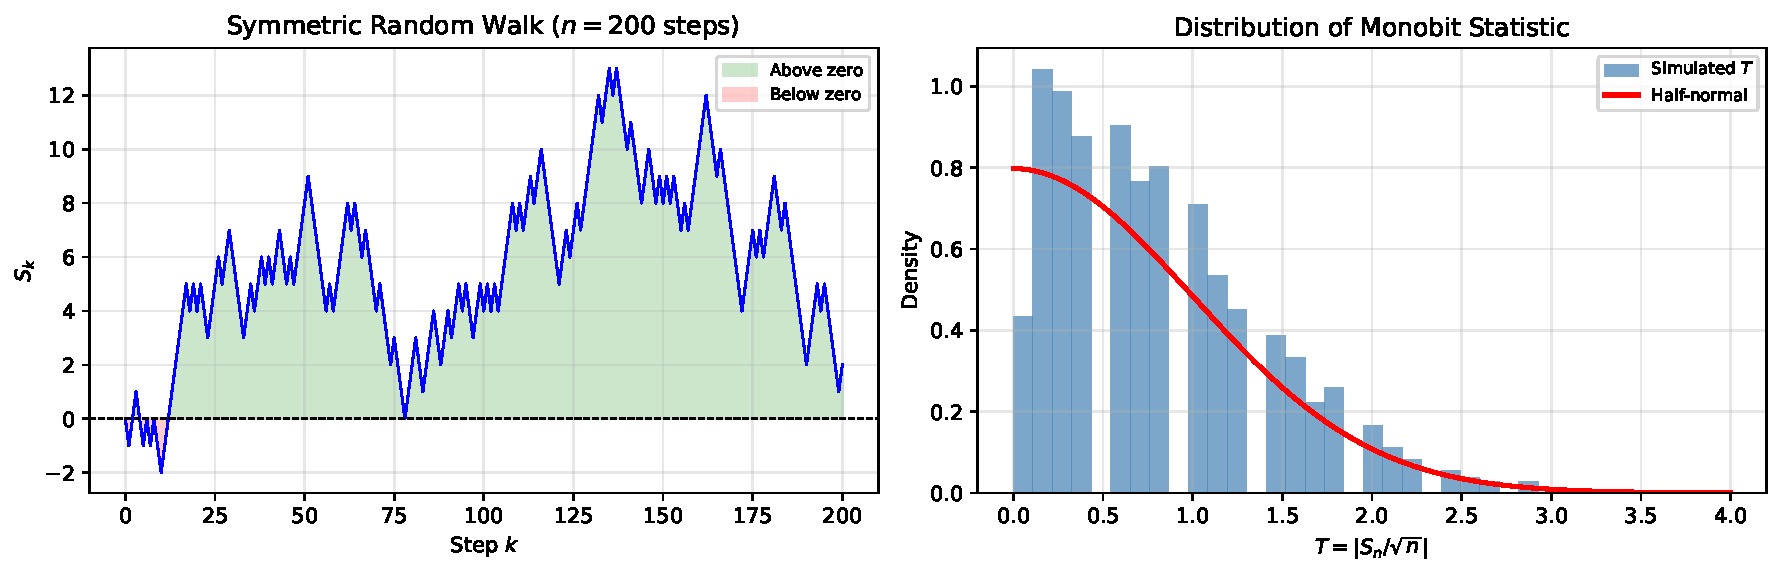
\includegraphics[width=0.80\textwidth]{random_walk}
\end{center}

\framebreak

\begin{block}{Frequency (Monobit) Test}
By the CLT: $S_n/\sqrt{n} \xrightarrow{\mathcal{D}} \mathcal{N}(0,1)$.\\
Test statistic: $T(\text{obs}) = |S_n/\sqrt{n}|$ follows a half-normal distribution.
\[
  p = \mathrm{erfc}\!\left(\frac{T(\text{obs})}{\sqrt{2}}\right),
\]
where $\mathrm{erfc}(x) = 1 - \mathrm{erf}(x) = \frac{2}{\sqrt{\pi}}\int_x^\infty e^{-t^2}\,dt$.
\end{block}

\medskip
\begin{block}{Frequency Test in Blocks}
Split $n = mr$ bits into $r$ blocks of length $m$. For each block $i$:
\[
  Z_i = \frac{S_m^{(i)}}{\sqrt{m}} = \frac{1}{\sqrt{m}}\sum_{j=1}^m (2B_{(i-1)m+j} - 1).
\]
Statistic: $T(\text{obs}) = \frac{1}{m}\sum_{i=1}^r (S_m^{(i)})^2 \approx \chi^2_r$.
\end{block}

\framebreak

\begin{block}{Arcsine Law Based Test}
Let $L_{2r}^+$ = number of steps $k$ where $S_k > 0$ (or $S_{k-1} > 0$) in a $2r$-step walk.
\textbf{Arcsine law:}
\[
  \lim_{r\to\infty} \mathbb{P}\!\left(\frac{L_{2r}^+}{2r} \le w\right)
  = \frac{2}{\pi}\arcsin\!\sqrt{w}, \quad w\in[0,1].
\]
The density $\frac{2}{\pi}\arcsin\!\sqrt{w}$ is U-shaped: the walk spends most of
its time \emph{either} above or below zero.
\end{block}

\begin{center}
  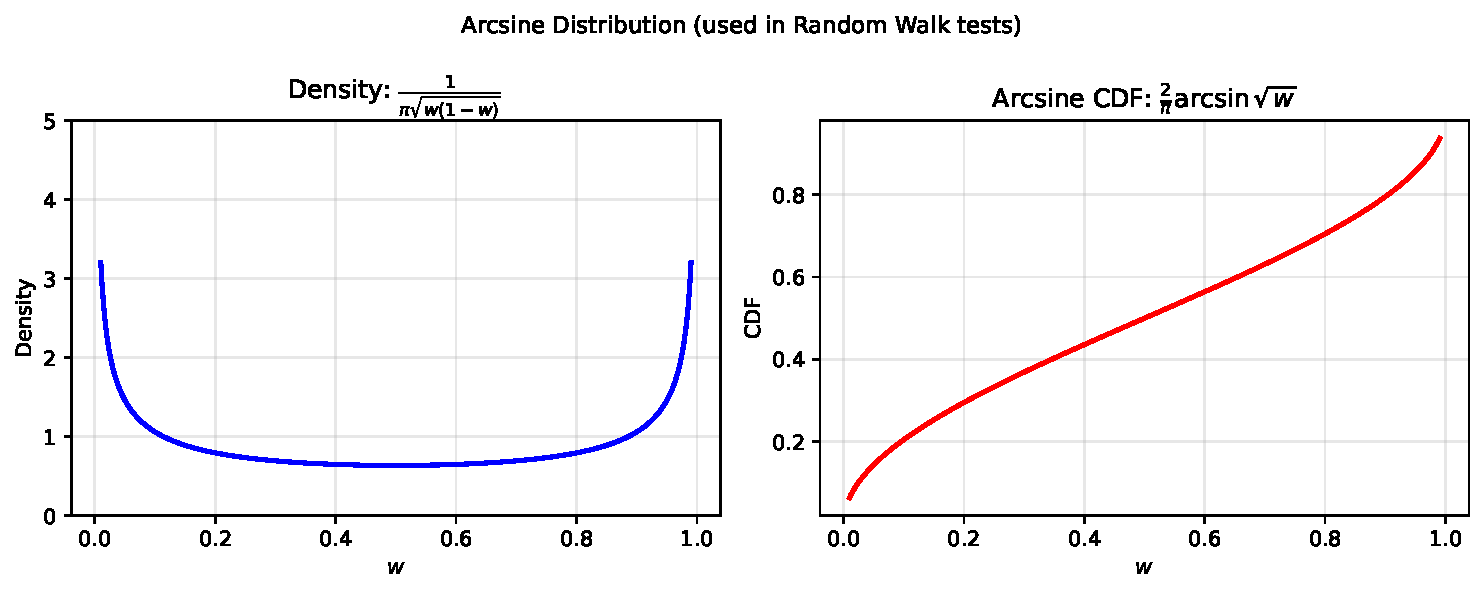
\includegraphics[width=0.60\textwidth]{arcsine_law}
\end{center}

Test: $T(\text{obs}) = \frac{1}{n}\sum_{k=1}^n d_k$ where $d_k = \mathbb{1}(S_k > 0 \vee S_{k-1} > 0)$.
$p$-value: $p \approx 1 - \frac{2}{\pi}\arcsin\!\sqrt{T(\text{obs})}$.

\framebreak

\begin{block}{Random Excursion Test}
Let $J_n$ = number of zeros (returns to 0) among $S_k$, $k=1,\ldots,n$.
Under $\mathcal{H}_0$:
\[
  \lim_{n\to\infty} \mathbb{P}\!\left(\frac{J_n}{\sqrt{n}} \le t\right)
  = \sqrt{\frac{2}{\pi}}\int_0^t e^{-x^2/2}\,dx.
\]
Reject if $J_n(\text{obs}) \le 0.008\sqrt{n}$ (NIST recommendation).
\end{block}

\medskip
\textbf{Distribution of visits per excursion:}
Let $L(x)$ = number of visits to $x$ during the 0th excursion.
\[
  \mathbb{P}(L(x)=k) = \begin{cases}
    1 - \frac{1}{2|x|}, & k=0,\\
    \frac{1}{4x^2}\left(1-\frac{1}{2|x|}\right)^{k-1}, & k \ge 1.
  \end{cases}
  \tag{2.5.22}
\]

\end{frame}

%% ------------------------------------------------------------------
\begin{frame}[allowframebreaks]{2.5.5 Permutation Tests}

\textbf{Derangement Permutation Test:}

\begin{block}{Definition: Derangement}
A \emph{derangement} of $[m] = \{1,\ldots,m\}$ is a permutation $\sigma$ with
\emph{no fixed points}: $\sigma(i) \ne i$ for all $i$.
\end{block}

\begin{block}{Lemma 2.5.10}
The number of derangements of $[m]$ is:
\[
  d_m = \sum_{k=0}^m (-1)^k \binom{m}{k}(m-k)! = m!\sum_{k=2}^m (-1)^k \frac{1}{k!}.
\]
As $m\to\infty$: $d_m/m! \to e^{-1} \approx 0.368$.
\end{block}

\framebreak

\textbf{Algorithm 3: Derangement Permutation Test}
\begin{enumerate}
  \item $\xi = 0$
  \item \textbf{for} $i=1$ to $r$:
  \item \quad $\sigma = $ Fisher-Yates$(m, (u_{(i-1)m+1},\ldots,u_{im}))$
  \item \quad \textbf{if} $\sigma$ is a derangement: $\xi = \xi + 1$
  \item Compute:
  \[
    T(\text{obs}) = \frac{|\xi - r e^{-1}|}{\sqrt{r e^{-1}(1-e^{-1})}},
    \quad p = \mathrm{erfc}\!\left(\frac{T(\text{obs})}{\sqrt{2}}\right).
  \]
\end{enumerate}

Under $\mathcal{H}_0$: $\mathbb{P}(\xi_i = 1) = e^{-1}$, so $\xi$ is binomial; CLT applies.

\framebreak

\textbf{Fixed Point Permutation Test:}

For each $m$-tuple $\mathbf{u}_i$, generate permutation $\sigma^i$ and count
$\xi_i = \#\{j : \sigma^i(j) = j\}$ (fixed points).

Under $\mathcal{H}_0$: $\xi_i \xrightarrow{\mathcal{D}} N$ (Poisson with mean 1) as $m\to\infty$.

\medskip
Use boxes $A_0 = \{0\}$, $A_1 = \{1\}$, \ldots, $A_9 = \{9\}$, $A_{10} = \{10,11,\ldots\}$.
Expected probabilities: $p_j = e^{-1}/j!$ for $j=0,\ldots,9$, $p_{10} = 1-\sum_{j=0}^9 p_j$.

Apply chi-square test with 10 degrees of freedom.

\end{frame}

%% ------------------------------------------------------------------
\begin{frame}[fragile]{2.5.5 Python Code: Permutation Tests}

\begin{lstlisting}[style=python]
import numpy as np
from scipy import stats

def fisher_yates(m, u):
    """Generate permutation of {0,...,m-1} from u in [0,1)^m."""
    S = list(range(m))
    for i in range(m, 0, -1):
        k = int(i * u[i-1])   # k in {0,...,i-1}
        S[k], S[i-1] = S[i-1], S[k]
    return S

def is_derangement(sigma):
    """True if sigma has no fixed points."""
    return all(sigma[i] != i for i in range(len(sigma)))

rng = np.random.default_rng(42)
m, r = 10, 1000     # m-tuples, r repetitions
n = m * r
u = rng.random(n)

xi = 0
for i in range(r):
    ui = u[i*m:(i+1)*m]
    sigma = fisher_yates(m, ui)
    if is_derangement(sigma):
        xi += 1

# Derangement test
e_inv = np.exp(-1)
T_obs = abs(xi - r*e_inv) / np.sqrt(r * e_inv * (1 - e_inv))
p_val = stats.erfc(T_obs / np.sqrt(2))
print(f"Derangements: {xi}/{r}, T={T_obs:.3f}, p={p_val:.4f}")
\end{lstlisting}

\end{frame}

%% ------------------------------------------------------------------
\begin{frame}[allowframebreaks]{2.5.6 p-Values and Second-Level Testing}

\textbf{Key insight:} Under $\mathcal{H}_0$ with a \emph{continuous} statistic $T$,
the $p$-value is itself $\mathcal{U}(0,1)$:
\[
  p = 1 - F(T(\text{obs})).
\]
\begin{block}{Proof sketch}
$\mathbb{P}(p \le t) = \mathbb{P}(1-F(T) \le t) = \mathbb{P}(T \ge F^{-1}(1-t)) = 1 - F(F^{-1}(1-t)) = t.$
\end{block}

\medskip
\textbf{Second-level testing procedure:}
\begin{enumerate}
  \item Split an $Rn$-length sequence into $R$ subsequences of length $n$
  \item For each subsequence $i$: compute statistic $T^{(i)}$ and $p^{(i)} = 1-F(T^{(i)})$
  \item Test uniformity of $p^{(1)},\ldots,p^{(R)}$ via chi-square:
    \begin{itemize}
      \item Partition $[0,1)$ into $s$ equal intervals: $P_i = [(i-1)/s, i/s)$
      \item $O_i = |\{j: p^{(j)} \in P_i\}|$, $E_i = R/s$
      \item $X^2_{\text{final}} = \sum_{i=1}^s (O_i - E_i)^2 / E_i \approx \chi^2_{s-1}$
    \end{itemize}
\end{enumerate}

\framebreak

\begin{center}
  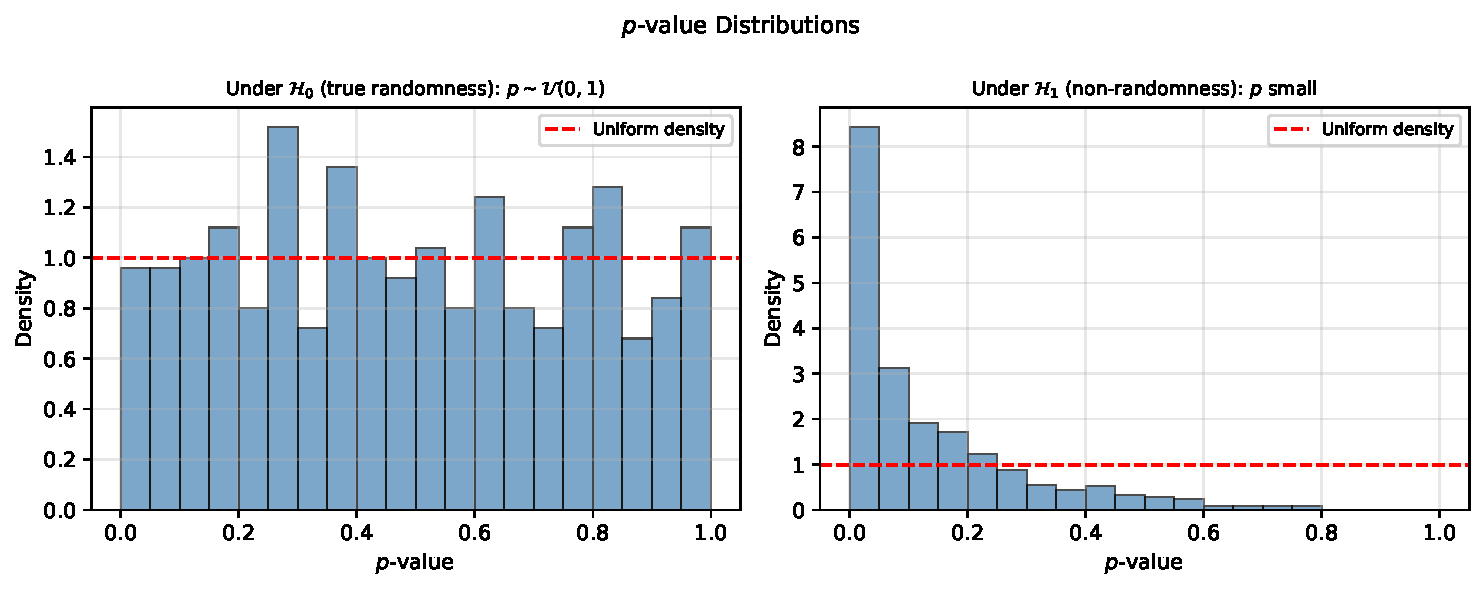
\includegraphics[width=0.80\textwidth]{pvalue_distribution}
\end{center}

\begin{center}
  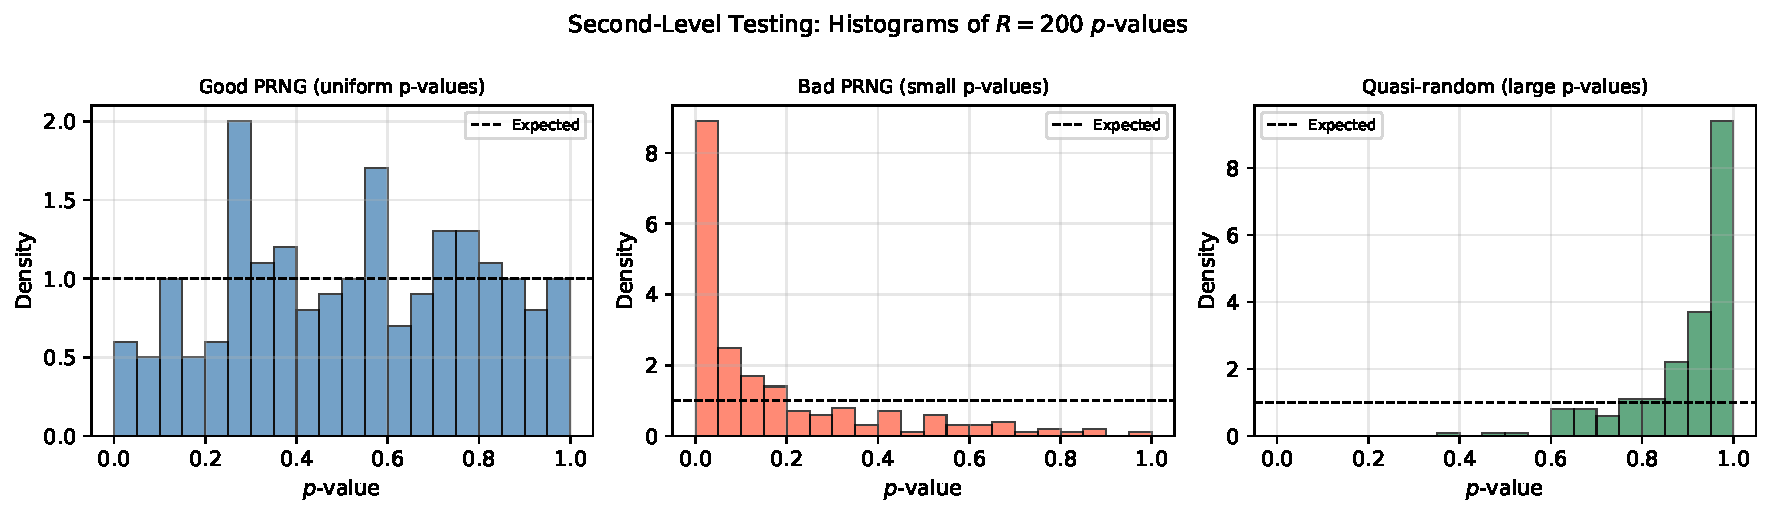
\includegraphics[width=0.80\textwidth]{second_level}
\end{center}

\framebreak

\textbf{Practical recommendations (NIST):}
\begin{itemize}
  \item Use $1000 \le R \le 10000$ sequences
  \item Sequence length $2^{20} \le n \le 2^{32}$
  \item Significance level $\alpha \in [1/1000, 1/100]$
  \item A PRNG passes if $\hat{B} \in [1-\alpha \pm 3\sqrt{\alpha(1-\alpha)/R}]$
    (fraction of sequences with $p > \alpha$)
\end{itemize}

\medskip
\textbf{Example 2.5.12:} Second-level KS and chi-square tests on sets A, B, C
with $R=200$ sequences of $n=50$.
\begin{itemize}
  \item Set A: $p$-values uniform --- passes
  \item Set B: $p$-values concentrated near 0 --- \textbf{fails}
  \item Set C (quasi-random): $p$-values concentrated near 1 --- \textbf{detected as non-random!}
\end{itemize}

Second-level testing \emph{detects} the ``too perfect'' uniformity of quasi-random sequences.

\end{frame}

%% ------------------------------------------------------------------
\begin{frame}[fragile]{2.5.6 Python Code: Second-Level Testing}

\begin{lstlisting}[style=python]
import numpy as np
from scipy import stats

def second_level_test(sequences, test_fn, s=10):
    """
    sequences: list of 1D arrays, each a subsequence
    test_fn: function returning p-value for a sequence
    s: number of bins for chi-square
    """
    p_vals = [test_fn(seq) for seq in sequences]
    # Chi-square uniformity test on p-values
    bins = np.linspace(0, 1, s+1)
    obs, _ = np.histogram(p_vals, bins=bins)
    exp = [len(p_vals) / s] * s
    chi2, p_final = stats.chisquare(obs, exp)
    return p_vals, chi2, p_final

# Generate R=200 sequences of n=50 from PCG64 (Set A)
rng = np.random.default_rng(0)
R, n = 200, 50
sequences_A = [rng.random(n) for _ in range(R)]

def ks_pvalue(seq):
    _, p = stats.kstest(seq, 'uniform')
    return p

p_vals, chi2, p_final = second_level_test(sequences_A, ks_pvalue)
print(f"Second-level KS test on Set A: chi2={chi2:.3f}, p={p_final:.4f}")

import matplotlib.pyplot as plt
plt.hist(p_vals, bins=20, range=(0,1), density=True, alpha=0.7)
plt.axhline(1, color='r', ls='--', label='Expected (uniform)')
plt.xlabel('p-value'); plt.ylabel('Density')
plt.legend(); plt.title('Second-Level Test: p-value Histogram')
plt.tight_layout()
\end{lstlisting}

\end{frame}

%% ==================================================================
\begin{frame}[allowframebreaks]{2.6 Bibliographical Notes}

\textbf{Foundational references:}
\begin{itemize}
  \item \textbf{Knuth} [107]: ``The Art of Computer Programming, Vol.\ 2'' ---
    comprehensive treatment of LCGs, period theory, and statistical tests
  \item \textbf{L'Ecuyer} [118, 122]: Theoretical and practical PRNG design;
    combined generators and TestU01 test suite
  \item \textbf{Marsaglia} [141, 145]: Diehard test battery; birthday spacing test;
    spectral tests
  \item \textbf{NIST SP 800-22} [187]: Statistical test suite for cryptographic PRNGs;
    15 standardized tests
\end{itemize}

\medskip
\textbf{Modern generators:}
\begin{itemize}
  \item \textbf{PCG64} (O'Neill [162]): Permuted Congruential Generators --- current
    NumPy default
  \item \textbf{MT19937} (Matsumoto \& Nishimura [146]): Mersenne Twister;
    period $2^{19937}-1$; passes Diehard but fails some TestU01 tests
  \item \textbf{AES-CTR}, \textbf{ChaCha20}: Cryptographically secure stream ciphers
\end{itemize}

\framebreak

\textbf{Shuffling and card mixing:}
\begin{itemize}
  \item \textbf{Bayer \& Diaconis} [14]: ``Trailing the Dovetail Shuffle to its
    Lair'' --- $\sim 7$ riffle shuffles needed for $n=52$ cards
  \item \textbf{Aldous \& Diaconis} [2]: Markov chain coupling methods for
    mixing time analysis
\end{itemize}

\medskip
\textbf{Theoretical test results:}
\begin{itemize}
  \item \textbf{Weiss} [210]: Normal approximation for empty boxes ($\mathcal{E}_{k,r}$)
  \item \textbf{Holst} [83], \textbf{L'Ecuyer et al.}\ [122]: Known results on the
    serial test chi-square statistic
  \item \textbf{Tsang et al.}\ [205]: Random excursion test analysis
  \item \textbf{L'Ecuyer \& Simard} [169, 170]: Reliable test design using
    Berry-Esseen bounds
\end{itemize}

\end{frame}

%% ==================================================================
\begin{frame}[allowframebreaks]{2.7 Exercises: Selected Problems}

\textbf{Theoretical exercises (sampling):}

\medskip
\textbf{2.T.1 (Markov and Chebyshev inequalities):}
\[
  \mathbb{P}(X \ge a) \le \frac{\mathbb{E}X}{a}, \quad
  \mathbb{P}(|X - \mathbb{E}X| \ge b) \le \frac{\mathrm{Var}X}{b^2}.
\]

\medskip
\textbf{2.T.4:} If $U_1,\ldots$ i.i.d.\ $\mathcal{U}(0,1)$ and $M \ge 2$, then
$\lfloor M U_i \rfloor$ is a random sequence from $\bar{M}$.

\medskip
\textbf{2.T.8:} Verify Fisher-Yates generates a uniform random permutation
(by induction on the swap steps).

\medskip
\textbf{2.T.17 (Serial test):} Show $\mathbb{E}X_k^2 = k-1$ for the serial test statistic.

\framebreak

\textbf{Lab exercises (sampling):}

\medskip
\textbf{2.L.1:} Implement LCG with $M=2^{11}-1$, $a=5$, $c=1$. Generate $10^4$
numbers, plot $(i, u_i)$ pairs. Find the period. Check Theorem 2.4.1.

\medskip
\textbf{2.L.2:} Compare Fisher-Yates vs.\ modified Algorithm B (where line 3 uses
$k = \text{random}(1,\ldots,n)$ instead of $\{1,\ldots,i\}$). Test with
fixed-point permutation test.

\medskip
\textbf{2.L.3:} Generate $n=10^5$ numbers with MT19937 and with LCG
($M=2^{31}-1$, $a=16807$). Compute the Pearson autocorrelation between
$(y_1,\ldots,y_{n-1})$ and $(y_2,\ldots,y_n)$.

\medskip
\textbf{2.L.5:} Quasi-random test: $u_i = i/M \bmod 1$ with $M=100$, $i=1,\ldots,10^6$.
Perform KS, chi-square, and second-level tests.

\end{frame}

%% ==================================================================
\begin{frame}{Chapter 2: Summary}

\begin{columns}
\column{0.5\textwidth}
\textbf{Key concepts covered:}
\begin{itemize}
  \item PRNG definition (5-tuple $(S,s_0,f,V,g)$)
  \item Random sequences: $\mathcal{U}(0,1)$, bits, integers
  \item Fisher-Yates shuffle; shuffling cards
  \item Python: \texttt{default\_rng}, PCG64, MT19937
  \item RC4 stream cipher (KSA + PRGA)
  \item LCG period conditions (Theorem 2.4.1)
  \item Bit generators: LFSR, XORG, SXR, BBS
\end{itemize}

\column{0.5\textwidth}
\textbf{Statistical testing:}
\begin{itemize}
  \item KS test: $D_n = \sup|\hat{F}_n - t|$
  \item Chi-square: $X^2 = \sum(O_i-E_i)^2/E_i$
  \item Balls-and-boxes: collision test, birthday spacing, poker test
  \item Random walk tests: monobit, arcsine law, excursion test
  \item Permutation tests: derangement, fixed-point
  \item Second-level testing: detect ``too perfect'' sequences
\end{itemize}
\end{columns}

\medskip
\begin{alertblock}{Take-home message}
No PRNG is perfect. Modern generators (PCG64) pass all practical tests,
but cryptographic applications require additional guarantees (AES-CTR, ChaCha20).
Always use second-level testing when verifying PRNG quality.
\end{alertblock}

\end{frame}

\end{document}
